\documentclass{beamer}
\usetheme[titlepagelogo=minerva2,% Logo for the first page
						language=italian
                        ]{TorinoTh}
                        
\usepackage[beamer,customcolors]{hf-tikz}
\hfsetfillcolor{alerted text.fg!10}
\hfsetbordercolor{alerted text.fg}

\author{Marco Odore}
\rel{Prof. Giorgio Valentini}
\assistantsupervisor{Dr. Marco Notaro}
\title[Metodi di Ensemble Gerarchici]{Metodi di Ensemble Gerarchici per la Predizione Strutturata della Funzione delle Proteine}
\ateneo{Università Degli Studi Di Milano}
\date{10 Luglio 2018}

\begin{document}
\titlepageframe
\begin{tframe}{Central Dogma}
  % 
  \begin{columns}
    %
    \begin{column}{.65\textwidth}
      \minipage[c][0.4\textheight][s]{\columnwidth}
	   \begin{itemize}	
	  \item All'interno delle molecole di DNA di ogni essere vivente esistono diverse migliaia di geni.   
      \onslide<2->
	  \item Si stima che per l'essere umano il DNA possegga tra i 20.000 - 25.000 geni.
      \onslide<3->
      \item Ogni gene all'interno del DNA è capace di codificare più proteine.	
      \onslide<4->
      \item Ogni proteina è responsabile di una o più funzioni all'interno delle cellule degli esseri viventi.
      \end{itemize}
      \endminipage      
    \end{column}
    %
    \begin{column}{.35\textwidth}

      % for top aligned images use minipage
      \only<1-4>{
        \minipage[c][0.4\textheight][s]{\columnwidth}

        \onslide<1->    

        \only<1-4>{
          \begin{figure}
            \centering
            \includegraphics<1>[scale=0.2]{img/DNA.png} %         
            \includegraphics<2>[scale=0.3]{img/humandna.png} %
            \includegraphics<3>[scale=0.2]{img/centraldogma.png}%
            \includegraphics<4>[scale=0.5]{img/funzioni.jpg}
        \end{figure}}


        \endminipage
      }   

      % for vertically centered images use parbox

    \end{column}
  \end{columns}

\end{tframe}

\begin{tframe}{La funzione delle proteine}


      Le proteine sono molecole biologiche composte da amminoacidi, e le funzioni che svolgono sono molteplici:
	   \begin{itemize}	
	   \onslide<2->
	   \item Metaboliche, ad esempio per la produzione di energia
	   \onslide<3->
		\item Di trascrizione, sintesi e processamento delle proteine stesse
		\onslide<4->		
		\item Di trasporto
		\onslide<5->
		\item Di comunicazione intra o intercellulare
		\onslide<6->
		\item Di ciclo della cellula, ad esempio per la divisione e riproduzione cellulare
      \end{itemize}
      \onslide<7->
      Per molte specie le funzioni di moltissimi geni (e quindi delle corrispettive proteine codificate) è \highlightbf{sconosciuta o parzialmente nota}.

\end{tframe}

\begin{tframe}{\small Il problema della predizione della funzione delle proteine 1/6}
  % 
  \begin{columns}
    %
    \begin{column}{.75\textwidth}
      \minipage[c][0.4\textheight][s]{\columnwidth}
	   \begin{itemize}	
	   \onslide<1->
	  \item L'individuazione della funzione delle proteine attraverso le analisi con sperimentazione diretta in laboratorio è \highlightbf{costosa} e richiede \highlightbf{molto tempo}
	  \onslide<2->
	  \item Esistono centinaia di funzioni a cui poter associare un gene/proteina \highlightbf{(problema multiclasse)}
	  \onslide<3->
	  \item Ad ogni gene/proteina possono essere associate diverse funzioni contemporaneamente \highlightbf{(problema multietichetta)}
      \onslide<4->
	  \item Il quantitativo di dati genomici cresce molto rapidamente.
      \end{itemize}
      \onslide<5->
      La \highlightbf{classificazione manuale} delle proteine è quindi infattibile.
      \endminipage      
    \end{column}
    %
    \begin{column}{.25\textwidth}

      % for top aligned images use minipage
      \only<1-5>{
        \minipage[c][0.4\textheight][s]{\columnwidth}

        \onslide<1->    

        \only<1-5>{
          \begin{figure}
            \centering
            \includegraphics<1>[scale=0.15]{img/lab3.jpg} %         
            \includegraphics<2>[scale=0.2]{img/multiclass.png} %
            \includegraphics<3>[scale=0.3]{img/multilabel.png}%
            \includegraphics<4->[scale=0.16]{img/growth.jpg}
        \end{figure}}


        \endminipage
      }   

      % for vertically centered images use parbox

    \end{column}
  \end{columns}

\end{tframe}

\begin{tframe}{\small Il problema della predizione della funzione delle proteine 2/6}
\begin{itemize}
\onslide<1->
\item A complicare ulteriormente il problema è il modo in cui sono \emph{relazionate} tra loro le funzioni delle proteine.
\onslide<2->
\item Esistono infatti due tassonomie principali per l'organizzazione delle classi:
\begin{itemize}

\onslide<3->
\item \highlightbf{Gene Ontology} (GO):  che organizza le funzioni come un grafo diretto aciclico (DAG), varia per ogni specie, e possiede tre ontologie differenti.
\onslide<4->
\item \highlightbf{Functional Catalogue} (FunCat): che è organizzato invece come un albero, non varia in base alle specie, e descrive le funzioni in maniera più sintetica rispetto alla Gene Ontology.
\end{itemize}

\end{itemize}  

\end{tframe}
\begin{tframe}{\small Il problema della predizione della funzione delle proteine  3/6}
\begin{figure}[h]
\center
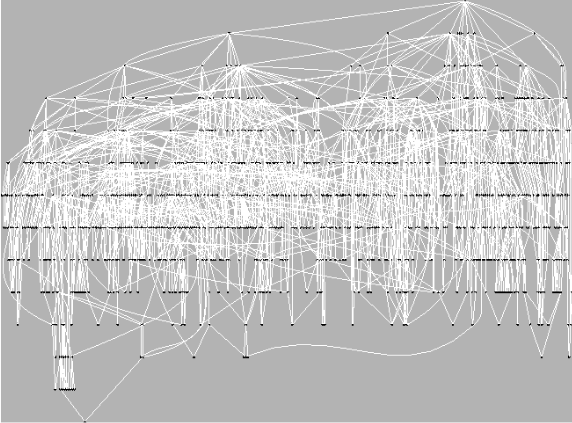
\includegraphics[scale=0.25]{./img/GO.png}
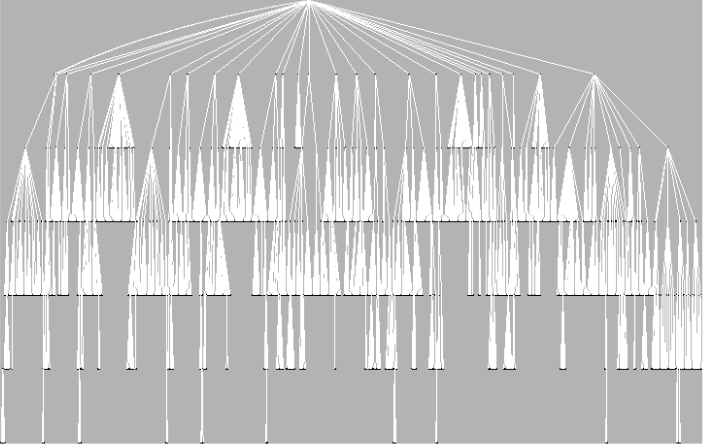
\includegraphics[scale=0.24]{./img/FunCat.png}
\caption{\footnotesize{A sinistra un DAG della GO per la specie \emph{S. cerevisiae}. A destra FunCat.}}
\label{DAGTREE}
\end{figure}
\end{tframe}


\begin{tframe}{\small Il problema della predizione della funzione delle proteine (GO) 4/6}
\begin{itemize}
\onslide<1->
\item Data la granularità e specificità superiori della GO e il suo largo utilizzo nella comunità scientifica, all’interno della tesi ci si è soffermati sulla predizione delle sue funzioni.
\onslide<2->
\item Tale tassonomia presenta tre ontologie (e quindi tre DAG) principali:
\begin{itemize}
\onslide<3->
\item \highlightbf{Processo Biologico} (BP): descrive i processi ad alto livello, come insieme di diverse attività molecolari.
\onslide<4->
\item \highlightbf{Funzione Molecolare} (MF): descrive le funzioni di specifici prodotti genici.
\onslide<5->
\item \highlightbf{Componente Cellulare} (CC): il luogo all’interno della cellula nelle quali avviene la funzione genica.
\end{itemize}
\end{itemize}  

\end{tframe}

\begin{tframe}{\small Il problema della predizione della funzione delle proteine (GO) 5/6}
Gli archi dei DAG nella GO indicano inoltre 3 differenti tipi di relazione:
\begin{itemize}
\onslide<2->
\item \highlight{is a}: indica una relazione di sotto-tipo.
\onslide<3->
\item \highlight{a part of}: indica una relazione di composizione
\onslide<4->
\item \highlight{regulates}: indica una relazione di influenza/regolazione
\end{itemize} 

\end{tframe}

\begin{tframe}{\small Il problema della predizione della funzione delle proteine (GO) 6/6}
\begin{figure}
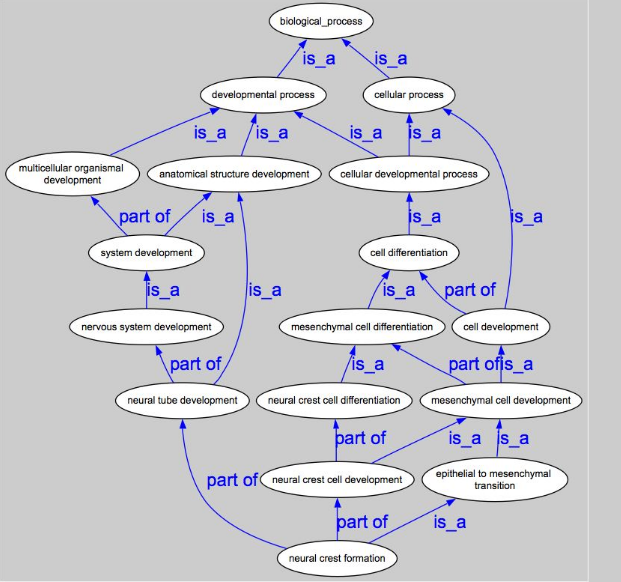
\includegraphics[scale=0.24]{./img/DAG_relations.png}
\caption{\footnotesize{Un porzione di DAG che evidenzia i diversi tipi di relazione.}}
\end{figure}
\end{tframe}

\begin{tframe}{\footnotesize{La predizione della funzione delle proteine tramite metodi automatici}}
Per gestire il problema della predizione della funzione delle proteine si rende quindi necessario un approccio \highlightbf{automatico}. I metodi più noti in letteratura sono:

\begin{itemize}
\onslide<2->
\item I metodi basati sulla \highlightbf{comparazione di biosequenze}: si basano sull'idea che sequenze simili condividano funzioni simili.
\onslide<3->
\item I metodi \highlightbf{basati su reti}: sono metodi applicati a dati rappresentati sotto forma di reti, che si basano sugli algoritmi di propagazione delle etichette.
\onslide<4->
\item I metodi \highlightbf{Kernel per spazi di output strutturato}: sono metodi che sfruttano funzioni kernel congiunte per predire in spazi di output strutturato.
\onslide<5->
\item I metodi \highlightbf{Ensemble Gerarchici}: i metodi trattati in questa tesi.
\end{itemize}

\end{tframe}

\begin{tframe}{Metodi Ensemble Gerarchici 1/3}
I Metodi di Ensemble Gerarchici sono metodi caratterizzati da due step principali:

\begin{enumerate}
\onslide<2->
\item \highlight{Predizione flat} delle diverse classi dell’ontologia, generando diversi predittori \emph{indipendenti}.
\onslide<3->
\item \highlight{Combinazione e correzione gerarchica delle predizioni} sfruttando il DAG dei termini della GO.
\end{enumerate}
\onslide<4->
Il secondo step rappresenta la componente \emph{ensemble} del metodo. Tale step si rende necessario in quanto le predizioni flat non tengono in considerazione la struttura gerarchica dei DAG della GO, portando a risultati \emph{inconsistenti}.

\end{tframe}
\begin{tframe}{Metodi Ensemble Gerarchici 2/3} 

\block{Consistenza \& True Path Rule}
Un insieme di predizioni $\hat{y} = <\hat{y}_1, \hat{y}_2, \dots, \hat{y}_{|N|}>$, dove $|N|$ è la cardinalità dei termini della gerarchia, è definito \emph{consistente}, se rispetta la \emph{True Path Rule}, e cioè:
\[
y\;\;\;consistente\;\; \leftrightarrow \forall i \in N, j \in par(i) \rightarrow y_j \geq y_i
\] 
Dove $par(i)$ indica l'insieme dei termini genitori del nodo $i$ nella gerarchia.
\endblock{}
\end{tframe}
\begin{tframe}{Metodi Ensemble Gerarchici (Esempio) 3/3}

\begin{center}
\includegraphics<1>[width=5cm]{img/1_1.png}
\includegraphics<2>[width=5cm]{img/2.png}
\includegraphics<3>[width=5cm]{img/3.png}
\includegraphics<4>[width=8.22cm]{img/4.png}
\end{center}
%\caption{Predittori flat indipendenti}


\end{tframe} 

\begin{tframe}{Metodi Ensemble Gerarchici: Approcci}
\begin{columns}
    \begin{column}{.50\textwidth}
      \minipage[c][0.4\textheight][s]{\columnwidth}
      Esistono fondamentalmente due approcci per la correzione:
	   \begin{itemize}
	   \onslide<2->
	  \item \highlight{Top-down}: le predizioni vengono corrette dai nodi più generali a quelli più specifici.
	   \onslide<3->	  
	  \item \highlight{Bottom-up}: Le predizioni vengono corrette dai nodi più specifici verso quelli più generali.
      \end{itemize}
      \endminipage 
    \end{column}
    %
    \begin{column}{.50\textwidth}
    \onslide<2-> 
        \minipage[c][0.4\textheight][s]{\columnwidth}
        \only<2-3>{
          \begin{figure}
            \centering
            \includegraphics<2>[scale=0.3]{img/topdown.png}
            \includegraphics<3>[scale=0.3]{img/bottomup.png}
        \end{figure}}
        \endminipage
    \end{column}
  \end{columns}
\end{tframe}

\end{document}
